\graphicspath{{Chapters/Chapter_ml-dataruns/}}

\chapter{Creating a randomized  dataset for training machine learning models}
\label{ch:ml-dataruns}

\section{Goal}

\section{The LAPD}

The Large Plasma Device (LAPD)\cite{gekelman_upgraded_2016,qian_design_2023} is a basic plasma science device located at the University of California, Los Angeles. The LAPD produces up to 18m long, 1m diameter plasmas  with densities up to $3 \times 10^{13}$ cm$^{-3}$ and temperatures up to 20 eV, though typical operation yields temperatures around 5 eV. Probes can sample virtually any point in this plasma through  unique ball valves placed every 32 cm along the length of the device, enabling the collection of time series data with high spatial resolution. The discharge repetition rate is configurable between 0.25 and 1 Hz. Additionally, the LAPD has 13 independently controllable magnet power supplies to shape the geometry of the axial magnetic field. The discharge is formed by 35 cm diameter lanthanum hexaboride (LaB6) cathode\cite{qian_design_2023} and 72 cm molybdenum anode 0.5m away (-z direction) at the southern end (+z) of the device. A cartoon of the LAPD and relevant coordinate system can be seen in Fig. \ref{fig:LAPD_coords}. 


The LAPD has many experimental control parameters for various physics studies. While the device can accommodate various insertable components, this study focuses on the parameters fundamental to the operation of the main cathode. Specifically, half way between the cathode and anode are three gas puff valves: East, West, and top. The aperture, duration, and triggering of these valves has a large impact on plasma formation. A static gas fill system also exists but it is not used in this study. The cathode-anode voltage (and consequently, discharge power) strongly influences plasma density and temperature downstream of the source. Additionally, the magnetic field configuration substantially shapes the plasma column. One crucial variable not considered in this study is the cathode temperature, as its adjustment and equilibration requires many hours, limiting dataset diversity. This combination of diagnostic coverage, high repetition rate, and extensive configurability renders the LAPD particularly suitable for machine learning studies. 

Data collection was conducted in two campaigns separated by 14 months. The initial run set is designated as \texttt{DR1} and the subsequent run set as \texttt{DR2}. These run sets are further broken down into \em dataruns \em which are series of discharges (``shots'') with identical operational machine parameters. A total of 67 dataruns were collected over both campaigns. 

The LAPD control parameters varied in this study were the source field, mirror field, midplane field, gas puff valve voltage, gas puff duration, and discharge voltage. The magnetic field regions are labeled in fig. \ref{fig:LAPD_coords} and effectively control the width of the plasma relative to the cathode in their respective regions. The gas puff voltage governs gas flow rate into the chamber, though this relationship is not yet quantified, and the gas puff duration defines the piezo valve activation period. The discharge voltage is applied across the cathode and anode 10 ms after gas puff initiation. While discharge voltage correlates to discharge current (and thus power), the current depends on the machine configuration and downstream conditions and cannot be predetermined.

These machine parameters -- with the exception of gas puff duration -- were randomly sampled via Latin-hypercube sampling (LHS) for 44 of the dataruns. Data were then collected with these settings. Gas puff duration was reduced for the last seven runs to 20, 10, or 5 ms (see fig. \ref{fig:PP1_time-series-example} for timings relative to $I_\text{sat}$ signals). The breakdown of each setting in the dataset is given in appendix \ref{sec:app_bias}, Table \ref{tab:data_frac}. The top gas puff valve was used for only the first nine dataruns of \texttt{DR2} because of equipment issues. 

$I_\text{sat}$ measurements were acquired along y=0 lines (51 dataruns total) or x-y grids (16 dataruns total) with spatial resolutions varying between 1.5 to 2 cm. The fixed axial locations of the probes were 895 cm and 831 in \texttt{DR1} and 1150, 1022, 863, and 639 cm for \texttt{DR2} (Fig. \ref{fig:LAPD_coords}). Six shots were recorded at each position except for the first four dataruns in \texttt{DR1} with five shots each.


\section{Data bias \label{sec:app_bias}}

Measurements over an x-y plane, constituting $\approx 64\%$ of all shots, are predominantly acquired overnight for maximal machine utilization. These longer dataruns lead to particular machine configurations being overrepresented in the dataset. 

The dataset predominantly contains gas puff durations of 38 ms. Only 6 runs in the training set have gas puff durations less than 38 ms: three have 5 ms and three have 10 ms, each having mirror ratios 1, 3, and 6 but otherwise identical configurations in an attempt to see mirror-related interchange instabilities in higher-temperature, lower-collisionality regimes. The 20 ms gas puff duration case is in the test set. This sampling bias towards the 38 ms gas puff duration suggests poor model performance is to be expected in shorter gas puff regimes. The top gas puff valve was operational for only the first nine runs of \texttt{DR2}.

\begin{figure*}
	\centering
	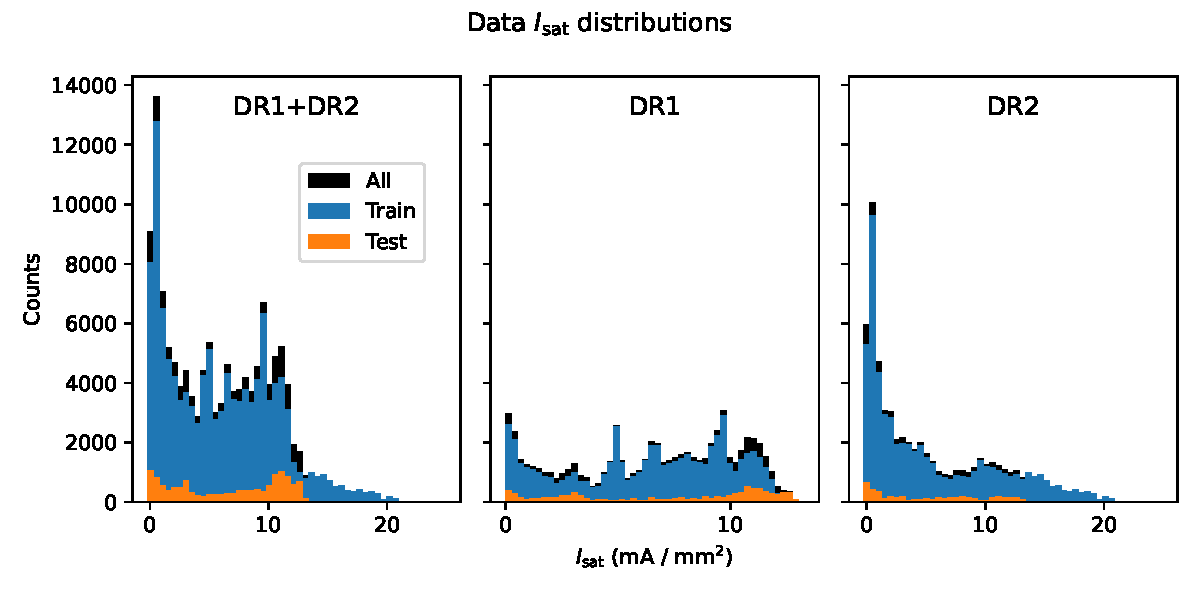
\includegraphics[width=\linewidth]{figures/PP1_02_isat_distribution.pdf}
	\caption[Time-averaged $I_\text{sat}$ distribution over shots]{\label{fig:PP1_02_isat_distribution}Distribution of $I_\text{sat}$ signals when averaged from 10 to 20 ms. \texttt{DR1} appears to have a more uniform distribution than \texttt{DR2} does. Combining the two datasets results in many $I_\text{sat}$ examples near 0 mA/mm$^2$ and a sharp decrease in number of examples above 10 mA/mm$^2$. From these histograms we expect or model to be biased towards fitting lower $I_\text{sat}$ values better, and to perform badly in cases with very high $I_\text{sat}$ values.}
\end{figure*}

Despite the best efforts to randomize the machine configuration, imbalance in the dataset will be present because of the relatively small amount of samples for the given actuator space. The distribution of $I_\text{sat}$ signals can be seen in Fig. \ref{fig:PP1_02_isat_distribution}. The $I_\text{sat}$ distribution is clearly different for \texttt{DR1} and \texttt{DR2}, with \texttt{DR1} having a much flatter distribution. These distributions imply that if the model is constrained to sample from \texttt{DR2} via the run set flag, then the model is expected to predict a lower $I_\text{sat}$ value in general. When predicting from the model in general, performance will likely be worse for $I_\text{sat}$ values $\gtrsim 11$ mA/mm$^2$. 

The $I_\text{sat}$ distribution is dissimilar between \texttt{DR1} and \texttt{DR2}: \texttt{DR1} appears to have a more uniform distribution. Combining the two datasets results in many $I_\text{sat}$ examples less than 2 mA/mm$^2$ and a sharp decrease in number of examples above 10 mA/mm$^2$. Thus, we expect the model to perform better for smaller $I_\text{sat}$ values than larger ones. Data bias is further discussed in section \ref{sec:app_bias}.


\begin{figure}
	\centering
	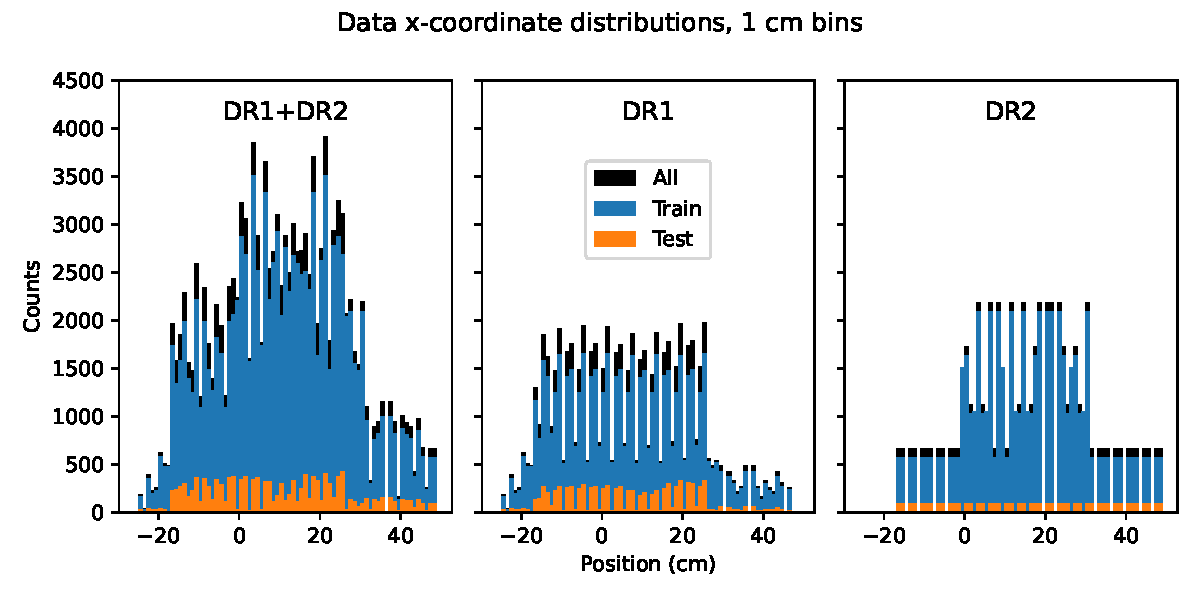
\includegraphics[width=\linewidth]{figures/PP1_02_x_distribution.pdf}
	\caption[Distribution of probe x-coordinates in the dataset]{\label{fig:PP1_02_x_distribution}Distribution of the x-coordinate in the profiles. The increase in data points between roughly x $\approx 0$ to 30 cm is from planes instead of lines. Based on this distribution, the performance of the model is expected to be biased towards this central area.}
\end{figure}

\begin{table*}
\small
	\centering
	\caption{Data breakdown by class and dataset (percent)}
	\label{tab:data_frac}
	\begin{tabular}{lrrr|lrrr|lrrr}
		\multicolumn{4}{c|}{B source (G)} & \multicolumn{4}{c|}{B mirror (G)} & \multicolumn{4}{c}{B midplane (G)}\\
		\hline \hline
		& Train & Test & All && Train & Test & All && Train & Test & All \\
%		\cline{2-4} \cline{6-8} \cline{10-12}
		500 & 4.77 & 0 & 4.29 & 250 & 4.30 & 8.41 & 4.72 & 250 & 8.25 & 21.01 & 9.55 \\
		750 & 3.34 & 12.61 & 4.29 & 500 & 30.49 & 8.41 & 28.23 & 500 & 43.80 & 8.41 & 40.19 \\
		1000 & 43.13 & 78.99 & 46.78 & 750 & 6.68 & 16.81 & 7.72 & 750 & 6.62 & 52.19 & 11.27 \\
		1250 & 12.59 & 0 & 11.30 & 1000 & 28.85 & 57.97 & 31.82 & 1000 & 26.36 & 5.78 & 24.26 \\
		1500 & 19.23 & 0 & 17.27 & 1250 & 3.34 & 4.20 & 3.43 & 1250 & 9.24 & 0 & 8.30 \\
		1750 & 1.91 & 0 & 1.71 & 1500 & 26.34 & 4.20 & 24.08 & 1500 & 5.73 & 12.61 & 6.43 \\
		2000 & 15.03 & 8.41 & 14.35 & & & & & & & & \\
		\\
		\multicolumn{4}{c|}{Gas puff voltage (V)} & \multicolumn{4}{c|}{Discharge voltage (V)} & \multicolumn{4}{c}{Axial probe position (cm)} \\
		\hline \hline
		70 & 12.11 & 16.81 & 12.59  & 70 & 12.22 & 8.41 & 11.83    & 639 & 12.48 & 8.41 & 12.06 \\
		75 & 6.68 & 0 & 6.00     & 80 & 5.25 & 0 & 4.72      & 828 & 17.07 & 36.28 & 19.03 \\
		80 & 11.46 & 8.41 & 11.15   & 90 & 2.86 & 8.41 & 3.43      & 859 & 12.48 & 8.41 & 12.06  \\
		82 & 41.49 & 57.97 & 43.17  & 100 & 3.34 & 8.41 & 3.86     & 895 & 33.01 & 30.10 & 32.71 \\
		85 & 14.13 & 0 & 12.69   & 110 & 8.77 & 0 & 7.87     & 1017 & 12.48 & 8.41 & 12.06 \\
		90 & 14.13 & 16.81 & 14.40  & 112 & 20.62 & 0 & 18.52   & 1145 & 12.48 & 8.41 & 12.06 \\
                      & & & & 120 & 3.82 & 8.41 & 4.29     &                       & & & \\
                      & & & & 130 & 0.95 & 0 & 0.86     &                       & & & \\
                      & & & & 140 & 2.86 & 8.41 & 3.43     &                       & & & \\
                      & & & & 150 & 39.30 & 57.97 & 41.20  &                       & & & \\
		\\
		\multicolumn{4}{c|}{Gas puff duration (ms)} & \multicolumn{4}{c}{Vertical probe position (cm)}\\
		\cline{0-7} \cline{0-7}
		$38$ & 94.27 & 91.59 & 94.00 & $\approx 0$ & 36.26 & 46.08 & 37.26 & \\
		$<38$ & 5.73 & 8.41 & 6.00    & $\neq 0$ & 63.74 & 53.92 & 62.74    & \\
		\multicolumn{12}{l}{}
	\end{tabular}
\end{table*}


The distribution of the selected machine settings for all the dataruns is enumerated in Table \ref{tab:data_frac}. Despite the randomization of the settings of 44 dataruns, the distribution is often uneven. This unevenness is exacerbated in the test set because that is a selection of 6 out of 67 dataruns. The remaining 23 non-random dataruns also contribute to the imbalance. For example, a source field of 1 kG and discharge voltage of 112 show up disproportionately in the dataset because data were collected at those settings while other equipment was being adjusted or calibrated.

%Another source of imbalance is the vertical location of the probe: overnight dataruns are often planar so that machine time can be effectively used, so there are fewer planar dataruns but with many more shots, leading to more shots having a nonzero y-coordinate. This imbalance could have been avoided if the LAPD had programmable machine settings; this capability may be developed in the future.

\section{Azimuthal asymmetry}

Examining the data, it appears that the y coordinate is not centered properly, possibly because the telescope used to align the probes is set incorrectly. Using profiles from planar data (see the ``before'' plot in fig. \ref{fig:y-alignment_before-after}), the y-coordinate was adjusted. The probes in DR1 were adjusted upwards by +2 cm. For DR2, the y-coordinate was adjusted separately for each probe. Port 17 was adjusted 6 cm up, port 21 was adjusted 4 cm up, port 26 was adjusted 4.5 cm up, and port 33 was adjusted 3.35 cm up. This degree of error is consistent with the centering scope crosshairs having some angle error, creating a larger absolute y-axis error closer to the cathode. An example of this y-axis error and the profile after shifting the coordinates can be seen in fig. \ref{fig:y-alignment_before-after}.

\begin{figure}
	\centering
	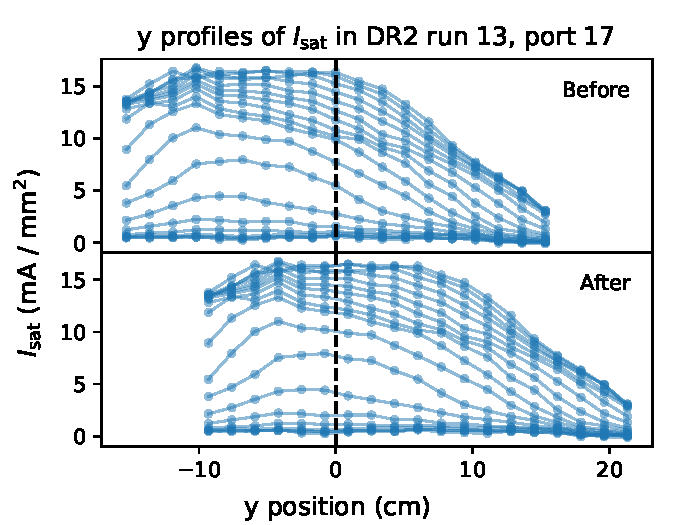
\includegraphics[width=300pt]{figures/y-alignment_before-after.pdf}
	\caption[y-axis profile before and after shifting the y-coordinate]{\label{fig:y-alignment_before-after}An example of the y-axis profile before and after shifting the y-coordinate. The ``before'' plot (top) is obviously asymmetrical about y=0. The shift needed to center was eyeballed from the plot. Each line represents a different x position, from closest to the core (upper lines) to the edge (lower lines).}
\end{figure}

